\documentclass[12pt]{article}
\usepackage[russian]{babel}
\usepackage{amssymb}
\usepackage{amsmath}
\usepackage{mathrsfs}
\usepackage[pdftex]{graphicx}
\usepackage[left=20mm, top=10mm, right=20mm, bottom=15mm]{geometry}
\usepackage{graphics}
\usepackage{gensymb}



\title{Лабораторная работа 1.4.2\\Определение ускорения свободного падения при помощи оборотного маятника}
\author{\textbf{Автор: Воробьев Игорь, Александр Егошин}}

\begin{document}
\maketitle
\textbf{Цель работы}: с помощью оборотного маятника измерить величину ускорения свободного падения.\\

\textbf{Оборудование}: оборотный маятник с двумя подвесными призмами и двумя грузами (чечевицами); электронный счётчик времени и числа колебаний; подставка с острием для определения положения центра масс маятника; закреплённая на стене консоль для подвешивания маятника; металлические линейки, штангенциркуль длиной 1 м.\\

\textbf{\large Теоретические сведения}


Физический маятник - твёрдое тело, способное совершать 
колебания в вертикальной плоскости, будучи подвешено за одну из своих 
точек в поле тяжести. Ось, проходящая через точку подвес перпендикулярно плоскости качания, называется осью качания маятника. 

При малых колебаниях период колебаний физического маятника определяется формулой: $$T = 2\pi\sqrt{\frac{I}{mgl}}\quad (1)$$


где I - момент инерциимаятника относительно оси качания, m - масса 
маятника, l -расстояние от оси качания до центра масс маятника. Если сравнить (1) с известной формулой колебаний математического 
маятника длиной l ($T = 2\pi\sqrt{\frac{l}{g}}$) определить приведённую длину физического маятника как: $$l_{\text{пр}} = \frac{I}{ml} \quad (2)$$

\begin{figure}[h!]
    \centering
    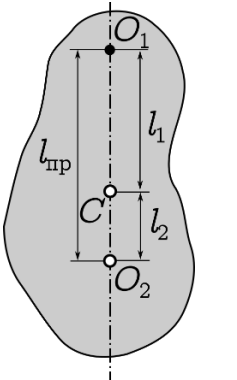
\includegraphics{Рис.1.png}
\end{figure}

где $l_{\text{пр}}$ - приведённая длина. Смысл приведённой длины в том, что при длине математического маятника, равной $l_{\text{пр}}$, его период колебаний совпадает с периодом колебаний физического маятника.\\


\textbf{Теорема Гюйгенса об оборотном маятнике}


Пусть $O_{1}$ - точка подвеса физического маятника, а 
C - его центр масс. Отложим отрезок длиной $l_{пр}$ вдоль 
линии $O_{1}C$, и обозначим соответствующую точку как $O_{2}$ — эту точку называют центром качания физического маятника. Заметим, что приведённая длина всегда больше расстояния до центра масс, поэтому точка $O_{2}$ лежит по другую сторону от центра масс.


Точки $O_{1}$ и $O_{2}$ обладают свойством взаимности: 
если перевернуть маятник и подвесить его за точку $O_{2}$
то его период малых колебаний останется таким же, как 
и при подвешивании за точку $O_{1}$.
$$T_{1} = 2\pi\sqrt{\frac{I_{1}}{mgl_{1}}}, \quad T_{2} = 2\pi\sqrt{\frac{I_{2}}{mgl_{2}}} \quad (3)$$
$$I_{1} = I_{c} + ml_{1}^2, \quad I_{2} = I_{c} + ml_{2}^2 \quad (4)$$
где $I_{c}$ - момент инерции относительно оси, проходящей через точку С.\\


\textbf{Измерение g}

Пусть $L=O_{1}O_{2}=l_{1}+l_{2}$. Если $T_{1}=T_{2}$, то $L=l_{\text{пр}}$. Из (1) и (2) находим ускорение свободного падения:
$$g_{0} = (2\pi)^2\frac{L}{T^2} \quad (5)$$

Точного совпадения $T_{1} = T_{2}$ на опыте добиться, конечно, невозможно. Поэтому получим формулу для определения ускорения свободного падения g, если измеренные периоды незначительно различаются: $T_{1}=T$ $T_{2}=T+\triangle T$. Из системы (3) и (4) получаем:
$$g=(2\pi)^2\frac{l_{1}^2 - l_{2}^2}{T_{1}^2l_{1}-T_{2}^2l_{2}} \quad (6)$$
что также можно переписать как
$$g=g_{0}\frac{\lambda - 1}{\lambda - \frac{T_{2}^2}{T_{1}^2}} \quad (7)$$
где $g_{0}=(2\pi)^2L/T^2$ и $\lambda = \frac{l_{1}}{l_{2}}$

Проанализируем отличия (5) и (7). Пусть $\varepsilon =\frac{\triangle T}{T}\ll 1$ - относительное отклонение при измерении периодов. Тогда при $\lambda \neq 1$, пользуясь малостью $\varepsilon$, получим
$$g=g_{0}\frac{\lambda - 1}{\lambda - (1+\varepsilon)^2} \thickapprox g_{0}\frac{1}{1 - \frac{2\varepsilon}{\lambda - 1}} \thickapprox g_{0}(1+2\beta\varepsilon)$$
где обозначено
$$\beta \equiv \frac{1}{\lambda-1} = \frac{l_{2}}{l_{1}-l_{2}}$$

Видно, что поправка $\triangle g \thickapprox 2\beta\varepsilon g$ к формуле (5) остаётся малой, если мало относительное различие измеренных периодов $\varepsilon$, но при этом также мал и коэффициент $\beta = \frac{l_{2}}{l_{1}-l_{2}}$. Поэтому на практике желательно, чтобы выполнялось $l_{1}/l_{2}>2,5$.\\

\textbf{Экспирементальная установка}

\begin{figure}[h!]
    \centering
    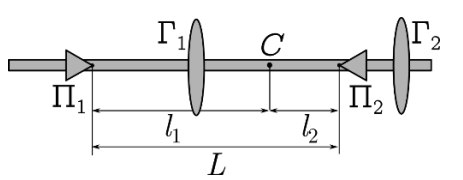
\includegraphics{2022-11-15.png}
\end{figure}
Применяемые в работе маятники представляет собой стержни цилиндрического или прямоугольного сечения длиной $\sim$ 1 м и массой $\sim$ 1÷1,5 кг. Маятник подвешивается с помощью небольших треугольных призм
(П1 и П2), острым основанием опирающихся на закреплённую на стене консоль. Ребро призмы задаёт ось качания маятника. На стержне закрепляются 
два дополнительных груза в форме «чечевицы» (Г1 и Г2). Для выполнения 
условия $l_{1}=l_{2}$ внешнюю чечевицу Г2 следует крепить за призмой П2, а чечевицу Г1 (внутреннюю) - между призмами П1 и П2.

Регистрация времени колебаний проводится с помощью электронных 
счётчиков. Расстояния между точками установки маятников на консоли до 
электронных счётчиков фиксировано.Фиксированное положение призм однозначно задаёт приведённую длину оборотного маятника $l_{\text{пр}} = L$\\

\textbf{\large Сбор данных}\\

$m_{\text{г1}}=1495,8$ г, $m_{\text{г2}}=1484$ г, $m_{\text{п1}}=78,9$ г, $m_{\text{п2}}=79,6$ г, $m_{\text{ст}}=868,3$ г, $\sigma_{m}=0,5$ г\\

$L_{\text{ст}}=1000,6$ мм, $L=607,5$ мм, $\sigma_{L}=0,1$ мм\\

С помощью  $\bot$-образной подставки удалось определить расположение центра масс маятника с грузами, он оказался удалённым от края со стороны груза Г2 на расстояние 372,7 мм.\\

Рассчитанный с помощью формулы \Large $\frac{\sum_{i}^n m_{i}x_{i}}{m_{i}}$ \normalsize центра масс был удалён от правого края на расстояние 373,2 мм. Таким образом, $l_{1}=432$ мм, а $l_{2}=175,5$ мм, $\sigma_{l}=1$ мм.\\

Колебания маятника при подвешивании за П2 (20 колебаний, отклонение \thickapprox 5\degree)\\

\begin{tabular}{c|c|c}
N & t,c & T,c\\
\hline
 1 & 31,22 & 1,561\\
 2 & 31,22 & 1,561\\
 3 & 31,14 & 1,557\\
 4 & 31,13 & 1,5565\\
\end{tabular}\\
\\

$T_{\text{ср}}$=1,558 c\\


Колебания маятника при подвешивании за П1 (20 колебаний, отклонение \thickapprox 5\degree)\\

\begin{tabular}{c|c|c}
N & t,c & T,c\\
\hline
 1 & 31,20 & 1,56\\
 2 & 31,20 & 1,56\\
 3 & 31,21 & 1,5605\\
 4 & 31,20 & 1,56\\
\end{tabular}\\

$T_{\text{ср}}$=1,56 c\\

Таким образом, \triangle T=0.002 \text{с},\; $\triangle T/T \thickapprox 0,001 $. Отклонение составляет около 0,1\%, что говорит о правильности определения положения грузов. Теперь проведём окончательное измерение периодов $T_{1}$ и $T_{2}$.\\

Колебания маятника при подвешивании за П2 (100 колебаний, отклонение \thickapprox 5\degree)\\

\begin{tabular}{c|c|c}
N & t,c & T,c\\
\hline
 1 & 155,52 & 1,5552\\
 2 & 155,5 & 1,555\\
 3 & 155,39 & 1,5539\\
\end{tabular}\\

Используя формулу среднеквадратичного отклонения $\sqrt{\frac{1}{n(n-1)}\sum_{i=1}^n(x_{i}-x_{\text{ср}})^2}$ получим, что $\sigma_{T2}^{\text{случ}}=0,0004$. Так как $\sigma_{T}^{\text{сист}}=0,001$с, получим, что $\sigma_{T2}\thickapprox 0,001$ c.\\

Колебания маятника при подвешивании за П1 (100 колебаний, отклонение \thickapprox 5\degree)\\

\begin{tabular}{c|c|c}
N & t,c & T,c\\
\hline
 1 & 155,99 & 1,5599\\
 2 & 155,97 & 1,5597\\
 3 & 156,02 & 1,5602\\
\end{tabular}\\

$\sigma_{T1}^{\text{случ}}=0,00015$ c, $\sigma_{T1}\thickapprox 0,001$ c.\\

Таким образом, $T_{1}=T=1,560\pm 0,001$ c, $T_{2}=T+\triangle T= 1,554\pm 0,001$ c.\\

\textbf{\large \text{Вычисление ускорения свободного падения}}\\

Воспользуемся формулой (6) для определения g, получим, что g=9.8187 м/с2. Для расчёта погрешности g воспользуемся формулой:
$$\sigma_{g} =g\sqrt{(\frac{\sigma_{L}}{L})^2+4(\frac{\sigma_{T}}{T})^2+8(\beta\frac{\sigma_{T}}{T})^2+8(\beta\frac{\triangle T}{T}\frac{\sigma_{L}}{\triangle l})^2} $$\\

где $\triangle l=l_{1}-l_{2}$ и $\triangle T=T_{1}-T_{2}$. Таким образом, получаем, что $\sigma_{g} = 0,0176$ м/с2 и \large $\frac{\sigma_{g}}{g}  \thickapprox 0,2\%.$\\

g\thickapprox9,82\pm 0,02\; \text{м/с2} \newpage\\

Можно рассчиать погрешность при расчётах по формуле (6), пользуясь стандартными правилами. Получим, что $\sigma_{g} = 0,0314$ м/с2, тогда $g\thickapprox9,82\pm0,03$ м/с2 и $\frac{\sigma_{g}}{g}\thickapprox0,3\%$.


\textbf{\large Вывод}\\

Нам удалось измерить с высокой точностью величину ускорения свободного падения за счёт использования оборотного маятника с двумя подвесными призмами и двумя грузами.

\end{document}
